%-----How to reach the lecture rooms
\section*{How to reach the lecture rooms}
\addcontentsline{toc}{section}{How to reach the lecture rooms}
The Conference has several locations: it will open in Aula magna Santa Lucia (via Castiglione 36).
Then on Tuesday 5 June afternoon and in the other days it will take place in:
\begin{itemize}
\item Building A and Building B - Room A, B, C, D, E, F, G, H, I, L, M, N, O, P, Q (via Belmeloro 14)
\item SP.I.S.A - Aula magna (via Belmeloro 12)
\item Redenti - Room 1 and Room 2 (via Belmeloro 10)
\item Matemates
\end{itemize}
The following map shows the location of these buildings

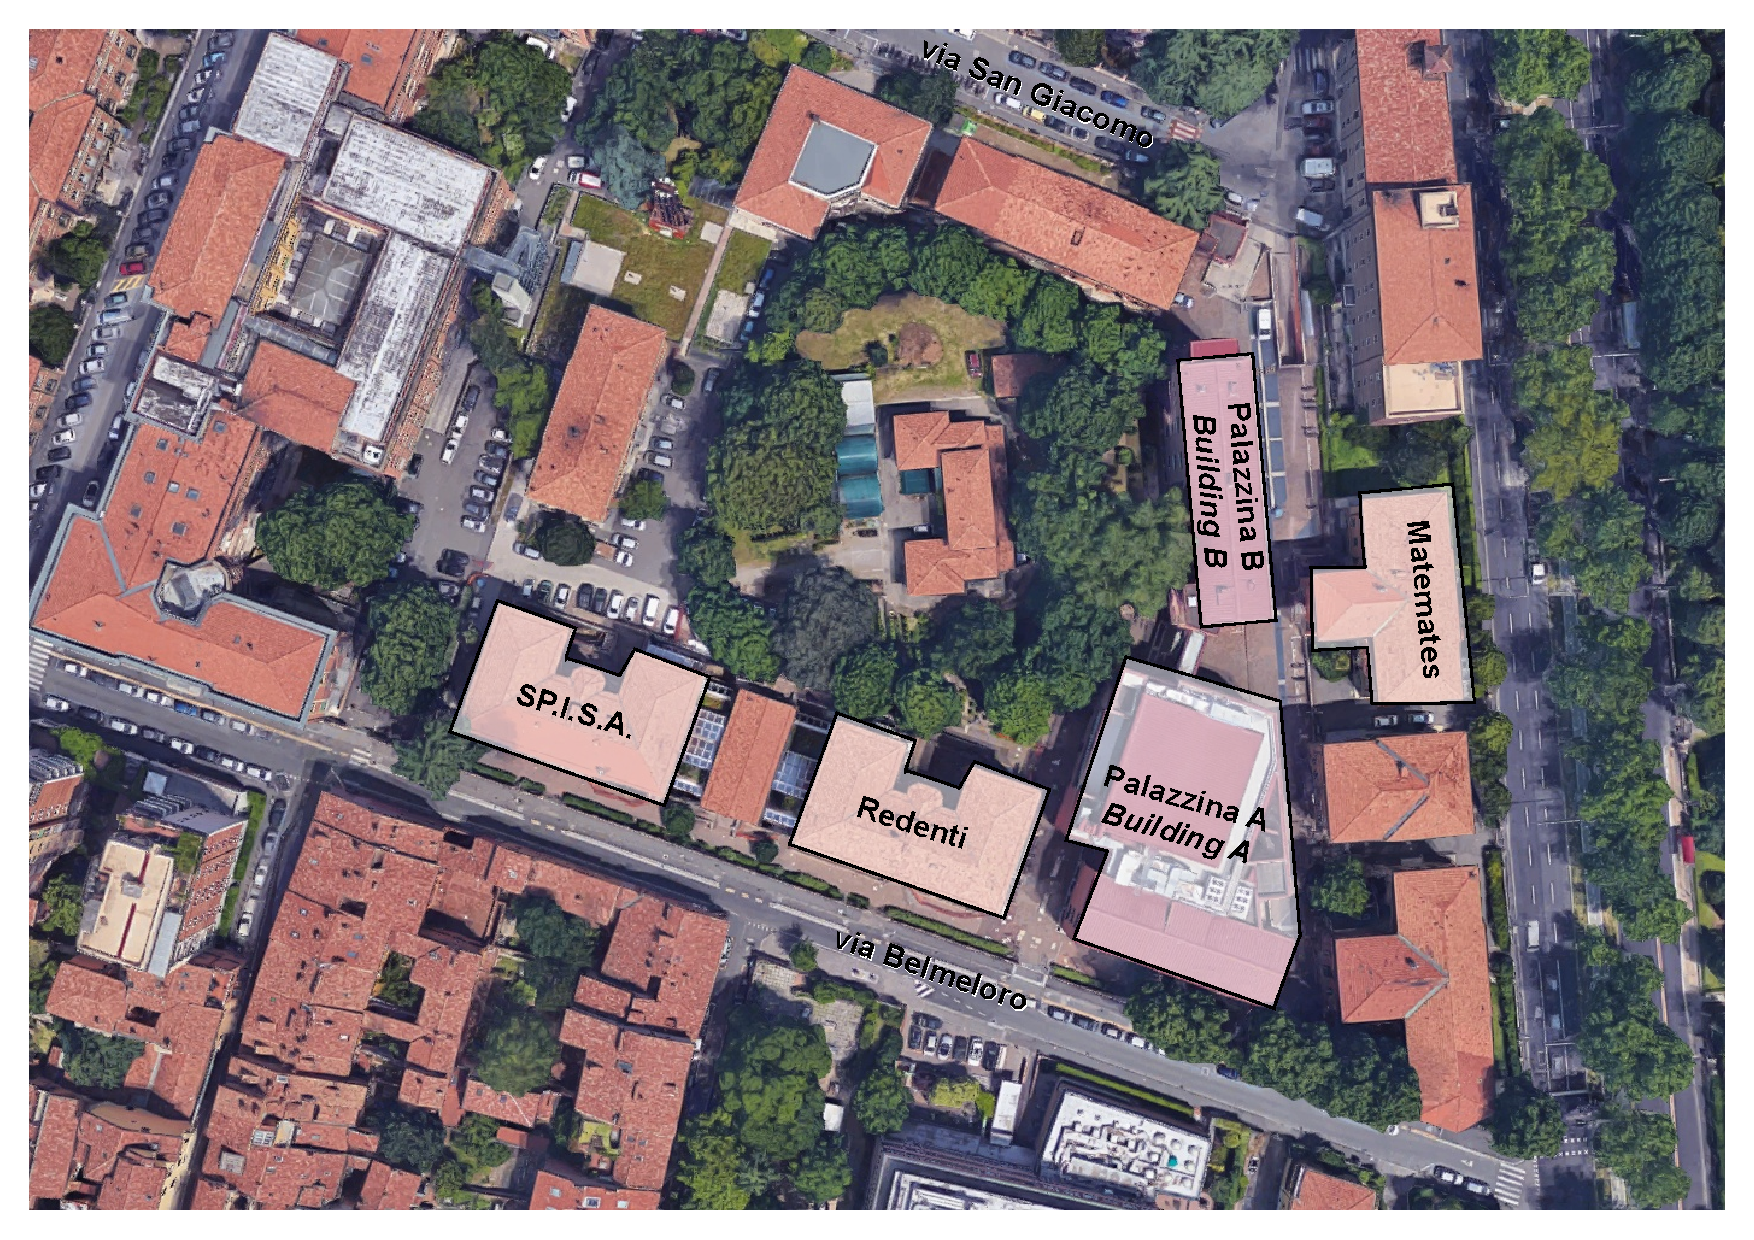
\includegraphics[scale=0.5]{satellite.pdf}
\newpage
\begin{center}
Building A and Building B (via Belmeloro 14) 
\end{center}
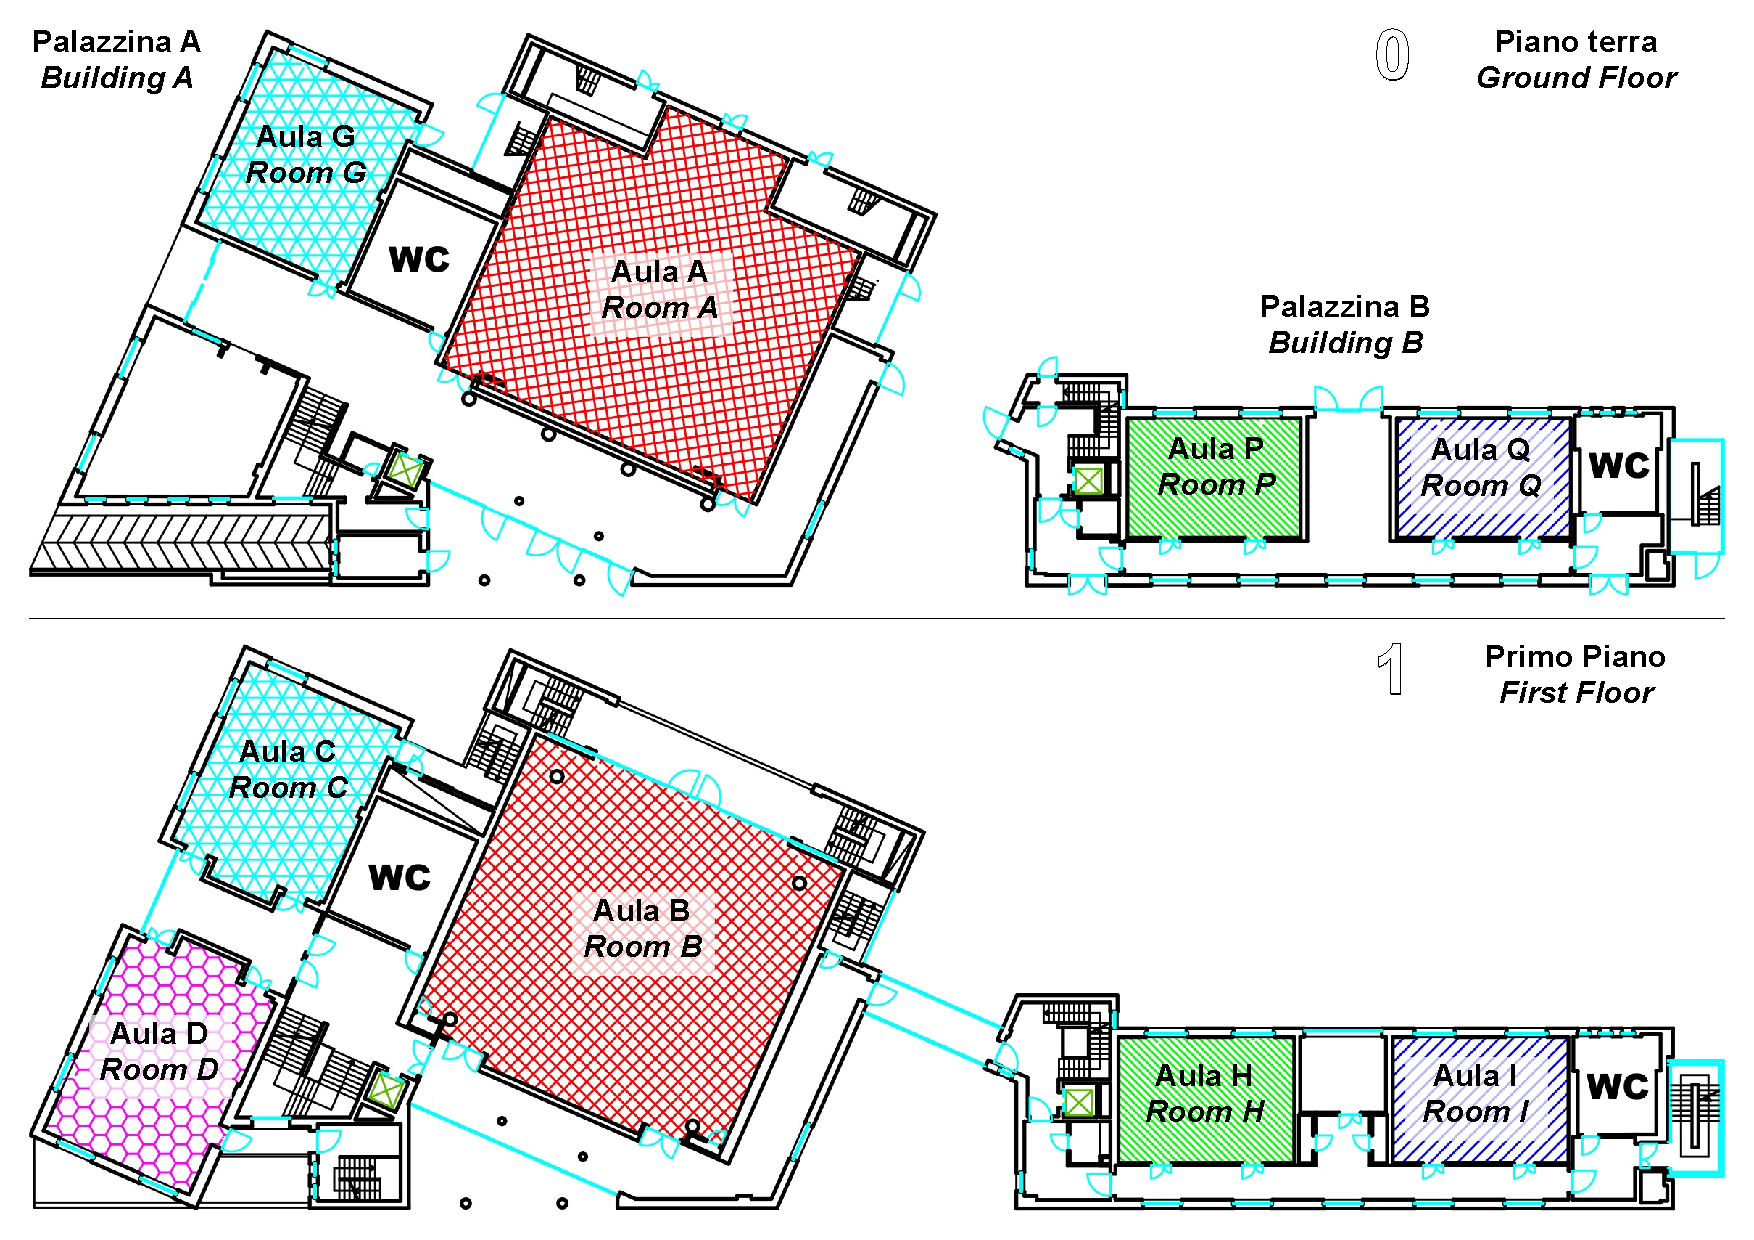
\includegraphics[scale=0.55]{Belmeloro14_floor0_1.pdf}

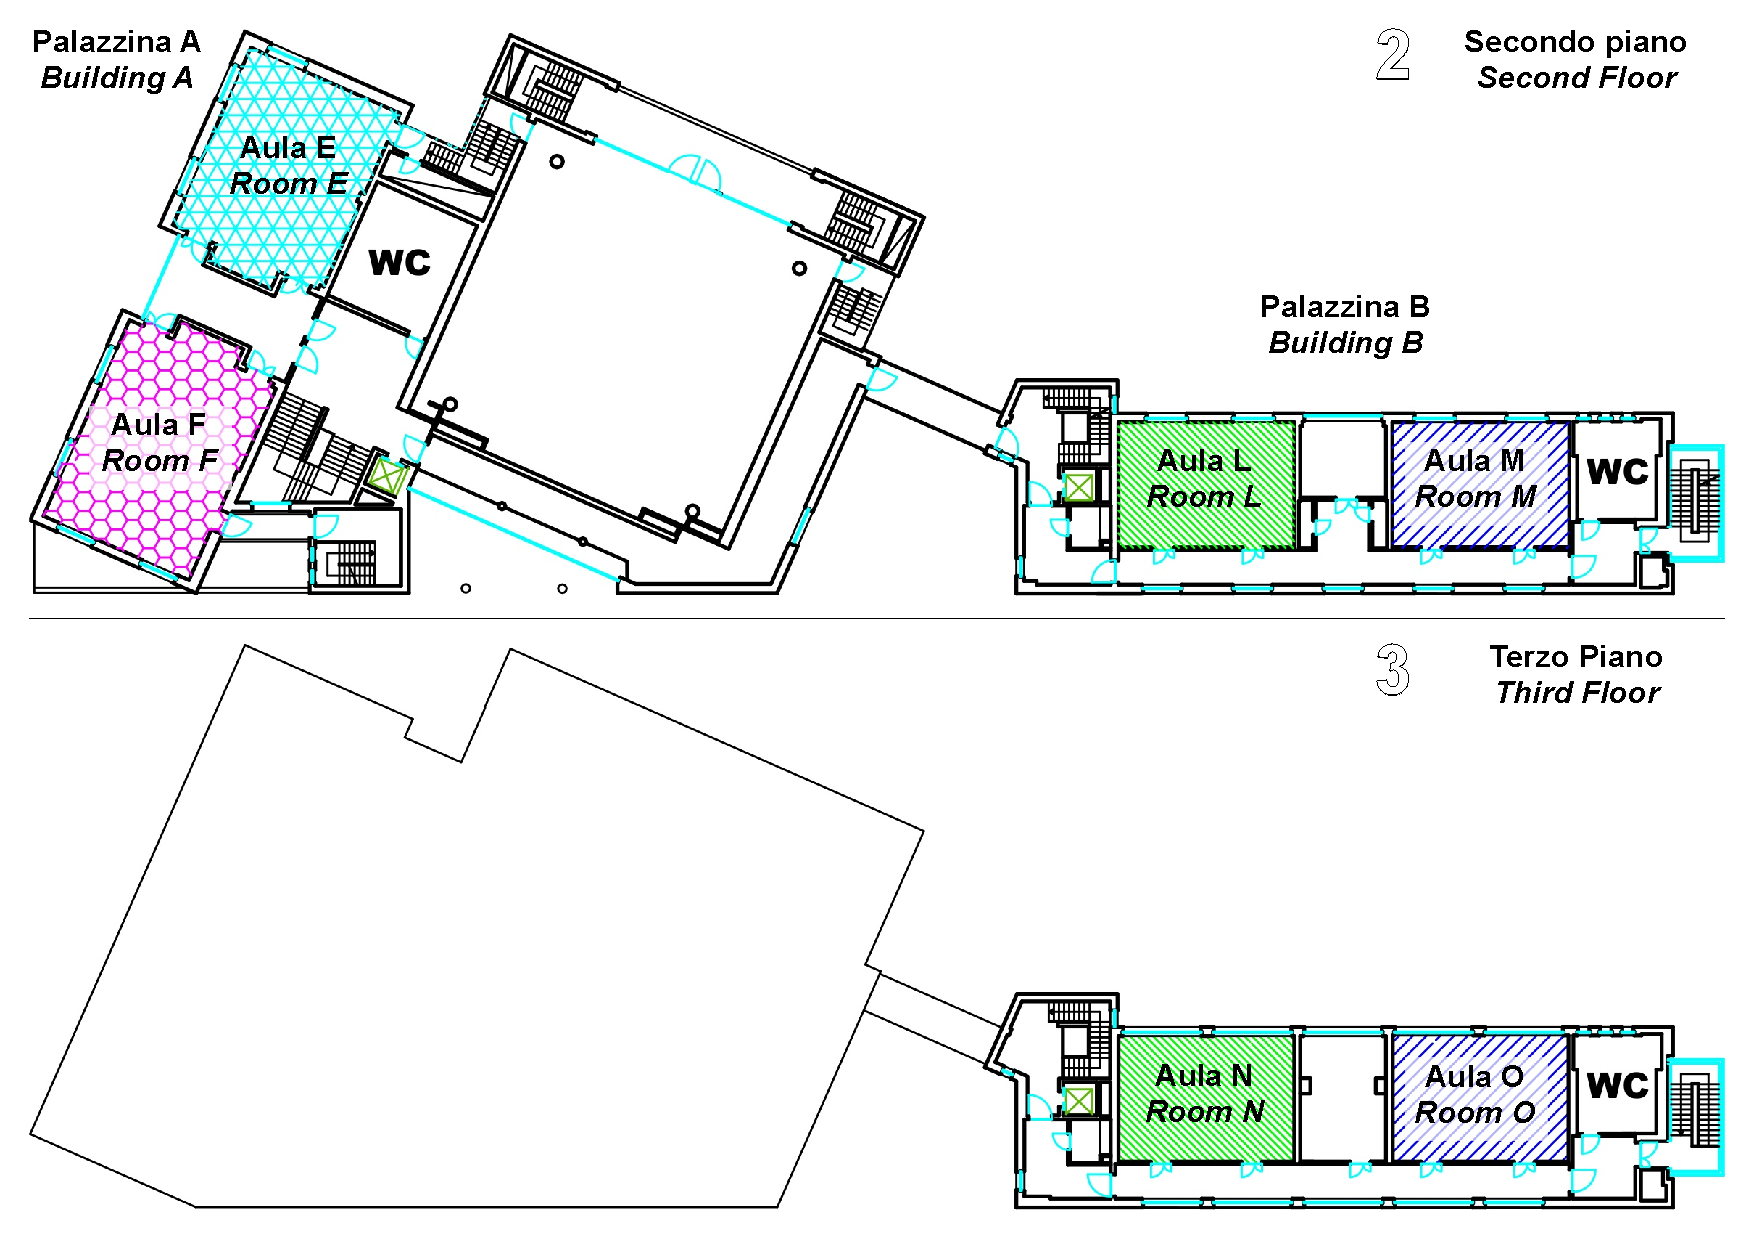
\includegraphics[scale=0.55]{Belmeloro14_floor2_3.pdf}
\begin{multicols}{2}
%-----Registration Desk
\section*{Registration Desk}
\addcontentsline{toc}{section}{Registration Desk}
The registration desk is located in the hall of Building A, via Belmeloro 14 and is open during the following hours:
\begin{itemize}
\item Monday, June 4: 3:00 PM - 6:00 PM
\item Tuesday, June 5: 12:00 PM - 6:30 PM
\item Wednesday, June 6: 8:30 AM - 6:30 PM
\item Thursday, June 7: 8:30 AM - 6:30 PM
\item Friday, June 8: 8:30 AM - 6:30 PM
\end{itemize}
%-----Name Badges
\subsection*{Name Badges} Carry your badge during the conference so that you can be admitted to all technical sessions, coffee breaks, lunches, reception and banquet (2014)\\
A space for emergency contact information is provided on the back of your name badge. Help us, help you in the event of an emergency! (2016)
%-----Registration Fee Includes
\subsection*{Registration Fee Includes}
\begin{itemize}
\item Admission to all technical sessions
\item Business Meeting (open to SIAG/IS members)
\item Social Dinner
\item Coffee breaks daily
\item Welcome Lunch and Poster Session
\item Room set-ups and audio/visual equipment
\item Wi-Fi access at the conference
\end{itemize}%-----Conference Talk Arrangements
%-----Conference Talk Arrangements
\subsection*{Conference Talk Arrangements}
All plenary talks will be 45 minutes in duration,
with 5 of the 45 minutes reserved for questions and discussion.\\\\
The minitutorials will be 2 hours in duration.\\\\
All minisymposia talks will be 30 minutes in duration, with 5 of the 30
minutes reserved for questions and discussion.
All contributed talks will be 20 minutes in duration, with 5 of the 20
minutes reserved for questions and discussion.\\\\
In case you need to copy your presentation slides from your USB to a
computer in lecture hall or meeting room, please do it in advance before
the session starts.
%-----Important Notice to Poster Presenters
\subsection*{Important Notice to Poster Presenters}
The poster sessions are scheduled for
\begin{itemize}
\item Tuesday, June 5 from 6:15 PM - 7:45 PM in Building A;
\item Wednesday, June 6 from 11:30 AM - 1:00 PM in Building A........
\end{itemize} 
The Best Poster Award will be assigned on Friday, June 8 at 1:00 in Building A, Room A.\\
All posters participating to the Best Poster Award are available on the Conference website.\\

Poster
presenters are requested to set up
their poster material on the provided
70 cm x 100 cm poster boards ........... 
All materials must
be posted by ??? at
5:00 PM, the official start time of
the session. Posters will remain on display through WHEN.
Posters displays must be removed by this time. Posters remaining after this time will be discarded.
The conference is not responsible for
discarded posters.
%------------Wi-Fi Access
\section*{Wi-Fi Access}
The username and password of your account during the conference period (5-8 June) can be found in your folder.
%-------------------Standard Audio/VIsual Set-Up in Meeting Rooms
\subsection*{Standard Audio/Visual Set-Up in Meeting Rooms}
The plenary session room has a PC, two screens and two data projectors.\\ 
All other concurrent/breakout rooms have a PC, a screen, a data projector and a whiteboard (overhead projectors are also available).\\
The data projectors support VGA connection only. Presenters requiring an HDMI or alternate connection must provide their own adaptor.\\
Cables or adaptors for Apple computers are not supplied, as they vary for each model: please bring your own cable/adaptor if using a Mac computer. 
The conference is not responsible for the safety and security of speakers' computers.\\
COME CI VOGLIAMO ORGANIZZARE???? Possono portare il loro computer? Vogliamo fare una cartella drive? 
%-------------Recording of presentations
\subsection*{Recording of Presentations}
Audio and video recording of presentations at the conference is prohibited without the written permission of the speaker and the conference.
%-------------SIAM Books and Journal
\subsection*{SIAM Books and Journals}CONTROLLARE
Display copies of books and complimentary copies of journals are available on site. SIAM books are available at a discounted price during the conference. The book booth will be staffed from 9:00 AM through 6:00 PM. \\If a SIAM books representative is temporarily away from the booth, completed order forms and payment (credit cards are preferred) may be taken to the registration desk. The books table will close at 4:00 PM on Friday??? (2016)\\
Completed order forms should be emailed or faxed to the SIAM office directly. It is not allowed to carry out on site transaction during the conference period??? (2014)
%------------------ GET TOGETHERS
\addcontentsline{toc}{section}{Get-togethers}
\subsection*{Get-togethers}
\begin{itemize}
\item Tuesday, June 5, 12:00 PM - 2:30 PM, Welcome Lunch
\item Tuesday, June 5, 6:15 PM - 7:45 PM, Poster Session I
\item Wednesday, June 6, 11:30 AM - 1:00 PM, Poster Session II
\item Thursday, June 7, 5:54 PM - 6:30PM, SIAG/IS Business Meeting
\end{itemize}
%---------------Lunches
\subsection*{Lunches}
Dove andare a pranzo
%---------------Conference Banquet
\subsection*{Conference Banquet}
The Conference banquet will be served in Palazzo Re Enzo, in Piazza del Nettuno 1C.\\ Additional conference banquet tickets are available: the price is 65 euros. Please check and buy at the registration desk before Tuesday, June 5 afternoon.
%---------------Child Care
\subsection*{Child Care}
\begin{itemize}
\item Le cicogne (http://www.lecicogne.net/)\\
Indicative rates: if reserved a few days in advance: \euro 16 / each hour (for a maximum of 2-3-4 hours) for a basic Baby Sitting and \euro 20/each hour for a Baby Sitter speaking foreign languages.
If requested one day before: \euro 18 + hourly rate.
If requested the same day: \euro 28 + hourly rate.
\item Born to life (http://www.bolognababysitter.it/)\\
Indicative rates: \euro 25 agency fee + hourly rate \euro 13 . After 10 PM: \euro 15 Foreign languages ??available. Reservations: 2 weeks in advance.?
\end{itemize}
%---------------Please Note
\subsection*{Please note}
The conference is not responsible for the safety and security of participants' computers. Do not leave your laptop computers and personal thngs unattended. Please remember to turn off your cell phone, pagers, etc in all the sessions.\\\\ The conference cannot provide photocopying and dollar exchange service. The bank can be found in piazza Aldrovandi 12/A.
%---------------Comments
\subsection*{Comments?}
Comments about SIAM IS18 are encouraged! Please send it to Cynthia Phillips, SIAM Vice President for Programs (vpp@siam.org)
\end{multicols}
